\begin{abstract}
Transparent transaction histories do not directly explain how a large wallet population behaves, and an unsupervised partition is not evidence of a natural taxonomy. This study develops a layered validation framework for Ethereum wallet segmentation under explicit historical cohort and feature-representation controls. Starting from an annual feature-table universe of 2,738,243 addresses, a complete historical code scan retains 2,508,997 addresses with empty code at the final Ethereum block of 2022. We construct a 16-feature count/activity/direction representation, excluding pooled ERC-20 amount magnitudes, and compare annual K2--K6 models across three initializations. Annual K3 provides a stable working resolution, with adjusted Rand indices of 0.908--0.971, while matched-estimator feature holdouts reveal substantial representation dependence. Shared transfer samples support 84 monthly network comparisons with 9,999 common label permutations and a global Holm correction. K3, K4 and K5 have above-null concentration in all twelve months, although K4 has larger network excess and lower initialization stability. Separate frozen monthly K2--K6 models, trained on January--June and evaluated on July--December, show above-chance persistence. K3--K6 also exhibit above-null conditional two-step return after correction across twenty tests; the binary K2 return null is structurally uninformative. The results support a qualified behavioural description rather than permanent EOA identities or a uniquely optimal cluster count. We provide a reproducible account of cohort construction, sensitivity, network alignment and temporal structure, including explicit limits on economic, causal and population-wide interpretation.
\end{abstract}

\begin{IEEEkeywords}
Ethereum, wallet segmentation, behavioural states, historical cohort, clustering validation, transaction networks, temporal analysis
\end{IEEEkeywords}

\section{Introduction}
Public blockchains expose detailed records of interactions, but accessibility is not the same as interpretability. A block explorer can describe an address or transaction, whereas a population-level explanation requires a vocabulary for differences in activity, direction and timing. In Ethereum, one address may interact intermittently over many months, another may concentrate a comparable number of transfers into one week, and another may remain active throughout the year. Aggregation can conceal these differences, while an unrestricted catalogue of individual histories is too large to provide a useful summary.

Wallet segmentation offers one descriptive approach. Addresses are represented by behavioural features and grouped according to similarity in that representation. Unlike ownership clustering or supervised entity classification, the aim is not to identify a controller, exchange, malicious actor or real-world user. The object of interest is the observable address-level activity pattern. Prior work establishes that transaction behaviour and graph structure can be informative for linkage, profiling and classification \cite{victor2020address,beres2021blockchain,bonifazi2022userspectra}; it does not establish that any particular unsupervised partition is a meaningful wallet taxonomy.

A cluster assignment alone does not establish a behavioural taxonomy. We evaluate geometric separation, initialization agreement, feature sensitivity, network alignment and held-out temporal structure as distinct claims. A stable partition can still depend strongly on its representation; a favourable internal score is not external validation \cite{halkidi2001validation,liu2022stability}.

Two controls motivate the redesign. A present-day code query does not establish historical EOA status, and pooled ERC-20 amounts lack a common economic unit without token-aware normalization. We use an explicit year-end code-free cohort and exclude pooled token amounts from the annual representation.

Our question is: \emph{can Ethereum addresses be organized into interpretable behavioural states under cohort, initialization, feature-family, network and temporal checks?} Annual roles and monthly states use different feature spaces. Neither constitutes a verified identity, and equal numerical labels do not establish correspondence.

The study contributes five linked components: a complete historical snapshot audit of the starting universe; a controlled 16-feature annual representation; K2--K6 initialization and feature-family comparisons; a shared-sample network validation with a declared multiple-testing family; and frozen, held-out monthly state models. K3 is a working annual resolution because its initialization stability and profiles provide an interpretable compromise. We also report the evidence that limits that choice, including K4's stronger average network excess and the feature dependence of K3 itself.

\section{Motivation}
\subsection{From Visible Transactions to Population Summaries}
Transaction records are observations of interactions, not ready-made behavioural categories. Counts, active days and temporal concentration summarize different aspects of a history. Two addresses with equal transfer totals can differ in duration, burstiness or direction. A population summary is useful when it preserves those distinctions while remaining understandable enough to inspect. This motivates a representation whose variables have concrete operational definitions rather than assigning economic or social meanings to unverified labels.

\subsection{Why Several Validation Layers Are Necessary}
Different checks address different failure modes. Initialization stability asks whether the solution is an accident of optimization. Feature-family removal asks whether an interpretation is dependent on a particular set of measurements. Network alignment asks whether labels relate to transfer endpoints under a specified randomization. Held-out monthly analysis asks whether a separately learned state representation captures structure outside its training months. None of these checks subsumes the others, and agreement between several layers does not make them statistically independent.

The need for separate layers is visible in the current results. Annual K4 has stronger mean network excess than K3 but much weaker initialization agreement. Monthly K2 has high persistence, but its conditional return test is degenerate. K3 is highly stable across annual seeds but changes substantially when activity or persistence features are removed. A single scalar ranking would conceal these differences. The objective is therefore a transparent evidence profile rather than a score that mechanically declares one partition universally superior.

\subsection{Behavioural States Without Identity Claims}
An address is not a person, and several addresses may be controlled by the same actor. Conversely, address-level activity can reflect interactions with applications or services rather than an individual preference. This study does not resolve those possibilities. The proposed names describe measured activity patterns: sustained activity, distributed lower activity and short-span concentrated activity. They are intended as readable summaries of profiles, not as externally verified classes such as traders, investors, bots or exchanges.

\section{Related Work}
\subsection{Address Linkage and Behavioural Classification}
Address-linkage research studies whether observed blockchain actions support inferences about common control or identity. Victor develops Ethereum address-clustering heuristics \cite{victor2020address}, while B\'{e}res et al. investigate profiling and deanonymization using graph and behavioural information \cite{beres2021blockchain}. These works establish the informational value of on-chain histories, but their inferential target differs from ours. We do not use a behavioural cluster to claim that addresses share ownership, nor do we evaluate identity recovery against labelled entities.

Bonifazi et al. describe user spectra using multivariate behavioural time series and classify users relative to predefined categories \cite{bonifazi2022userspectra}. Their use of temporal representations motivates treating behaviour as an evolving observation rather than a fixed attribute. The distinction is that our annual and monthly categories are learned without category labels. Interpretability must therefore be assessed through measured profiles and sensitivity, rather than inferred from agreement with a pre-existing semantic class.

\subsection{Temporal and Network Perspectives}
Ethereum interaction analysis also uses temporal graph properties and network representations. Agarwal et al. examine malicious-account detection through temporal graph properties \cite{agarwal2021temporal}, and T-EDGE develops temporal weighted multidigraph embeddings \cite{tedge2020}. Liang et al. study evolving cryptocurrency transaction networks \cite{liang2018evolutionary}. These studies motivate examining interactions and temporal dependence alongside feature-space similarity, without implying that network communities and behavioural roles must coincide.

Our network statistic is deliberately simpler than a community-detection objective. We compare the fraction of within-cohort transfers joining equal annual labels with a wallet-label permutation baseline. The test preserves the sampled interactions but destroys label--wallet association. This establishes a specific form of label--network alignment when the observed fraction exceeds the null. It neither estimates a latent interaction mechanism nor controls every structural property that could explain the alignment, particularly the relationship between behavioural labels and endpoint degree.

\subsection{Validation of Unsupervised Partitions}
Clustering validation distinguishes compactness, agreement and substantive usefulness \cite{halkidi2001validation}. Stability reviews emphasize that perturbation choices determine what a stability result means \cite{liu2022stability}. We therefore separate seed perturbations from feature removal and temporal evaluation. ARI and NMI compare partitions without relying on arbitrary label numbers \cite{hubert1985partitions,vinh2010information}; Hungarian matching provides a complementary address-level agreement \cite{kuhn1955hungarian}. Silhouette describes internal separation but is not treated as an estimator of a unique true number of wallet types \cite{rousseeuw1987silhouettes}.

\section{Methodology}
\subsection{Study Design and Validation Layers}
The pipeline begins with the fixed annual address universe and historical code observations. The retained membership is then shared across annual feature analysis, transfer-network filtering and monthly state analysis. The annual branch uses sixteen aggregate features, while the monthly branch uses six within-month count features. Transfer records provide a separate interaction view. Figure~\ref{fig:pipeline} summarizes this separation, and Table~\ref{tab:layers} identifies the claim supported by each layer.

\begin{figure*}[t]
\centering
\fbox{\parbox{0.94\textwidth}{\centering
\textbf{Fixed annual feature universe: 2,738,243 addresses}\\[3pt]
$\downarrow$ Historical code at block 16,308,189; complete evidence for every candidate\\[3pt]
\textbf{Year-end code-free cohort: 2,508,997 addresses}\\[5pt]
\begin{tabular}{p{0.29\textwidth}p{0.29\textwidth}p{0.29\textwidth}}
\textbf{Annual branch} & \textbf{Network branch} & \textbf{Monthly branch}\\
16 count/activity/direction features; K2--K6 and three seeds; matched K3 feature holdouts & Shared within-cohort transfer samples; seven annual label solutions; 84 permutation tests & Six count-only features; Jan--Jun training; frozen K2--K6 models; Jul--Dec persistence and return\\
\end{tabular}\\[5pt]
\textbf{Joint interpretation: stability, representation dependence, network alignment and conditional temporal structure}
}}
\caption{Controlled layered pipeline. Annual roles, network diagnostics and monthly state IDs are distinct analytical objects sharing a documented cohort.}
\label{fig:pipeline}
\end{figure*}

@@LAYER_TABLE@@

\subsection{Data Preparation and Historical Cohort Definition}
We use the 2022 ERC-20 transfer release from Harvard Dataverse and its dataset description \cite{somin2025erc2022,somin2025dataset}. The supplied annual feature table contains 2,738,243 addresses. This starting universe is a defined analytical population, not a census of every Ethereum address or every possible form of Ethereum use. All results are conditional on inclusion in that table. The network analysis reads 245,911,059 transfer rows from the twelve supplied monthly files, while the daily inputs supply wallet-level count histories for temporal modelling.

For each candidate address, the historical scan queries code at block 16,308,189, the final Ethereum block of 2022. The retained criterion is exactly empty code at this block. Every candidate has a resolved outcome: 2,508,997 are retained and 229,246 have nonempty code. No missing or failed query is converted into a code-free result. Membership is exported with a block identity and a checksum so that downstream steps can use the same population without repeating the RPC scan.

This rule is more temporally aligned with the study period than a present-day code query, but it remains a single-snapshot rule. Empty code at year-end does not establish continuous EOA identity throughout 2022, ownership, or code status at every transfer. We therefore use the term \emph{year-end code-free cohort}. The paper does not replace this operational definition with the stronger claim that all retained addresses were externally owned accounts throughout the observation period.

The historical list also changes the earlier retained population. The prior filter retained 2,443,868 addresses; the new list shares 2,443,852 of them, adds 65,145 previously excluded addresses and removes 16 previously retained addresses. The net increase is 65,129 addresses, or approximately 2.66\% of the old retained count. These differences should not be interpreted as the isolated effect of a cohort correction on the final clusters, because the main representation was also redesigned to exclude pooled token amounts.

@@COHORT_TABLE@@

\subsection{Source Validation and Reproducible Alignment}
All twelve wallet-day files are checked for valid normalized address identifiers, dates inside the expected month, finite nonnegative integer transaction counts, and unique wallet--day records. Duplicate normalized wallet--day rows are rejected even when the total row count is below the number of days in the month. A zero-count row does not add an active day. Address normalization removes an optional hexadecimal prefix and uses a consistent lowercase, forty-character representation before cohort joins.

Cohort membership and row order are checked separately. Annual manifests record feature-source and matrix hashes, column order, model settings and label hashes. Monthly cache signatures incorporate source contents, cohort and preprocessing code. Training wallet IDs are sorted before sampling so a fixed seed identifies a reproducible sample.

\subsection{Wallet-Level Feature Engineering}
The annual representation contains sixteen features in three declared families. Activity level includes observed wallet-day count, total transfer-record incidence, average daily count, maximum daily count and daily-count standard deviation. Persistence/concentration includes activity span, activity density, count coefficient of variation and transaction concentration. Directionality includes incoming-, outgoing- and both-active day counts, their three observed-day ratios, and directional day balance. Family removal uses this grouping; the analysis is not preregistered.

The annual source builder counts observed wallet-day rows. Annual mean and standard deviation use those observed days, whereas monthly calendar-day summaries also include absent days as zeros. Span is the inclusive first-to-last observed interval; density is observed days divided by span; concentration is maximum daily count divided by total count. Directional flags are defined by positive daily incoming or outgoing pooled amounts, not directional transfer counts. Thus zero-value events can contribute to count features without activating a directional flag. Amount magnitudes are excluded from the model, but directionality is not wholly independent of their preprocessing. Transfer counts denote wallet-record incidence, not distinct Ethereum transactions; the source conversion creates both sender and recipient records, including two incidences for a self-transfer.

Counts and durations are transformed with $\log(1+x)$ to reduce the geometric dominance of large raw magnitudes. Ratios, directional balance, count coefficient of variation and concentration remain in their original units before scaling. Each transformed column is centred by its full-cohort median and divided by its interquartile range. The resulting robust-scaled matrix has 2,508,997 rows and sixteen columns. Profiles are subsequently reported in raw units so that a transformed coordinate is not mistaken for a directly observed quantity.

For transformed feature $z_{ij}$ of address $i$ and column $j$, the representation used by the annual estimator is
\begin{equation}
 x_{ij}=\frac{z_{ij}-\operatorname{median}(z_{\cdot j})}{Q_{0.75}(z_{\cdot j})-Q_{0.25}(z_{\cdot j})}.
\end{equation}
The implementation uses a denominator of one if an interquartile range is zero. The input audit finds no nonfinite values in the sixteen retained annual columns. No amount magnitude, token-price feature, gas variable or identity label enters this matrix. A legacy cluster field retained in the source CSV for traceability is explicitly excluded from fitting. Seven direction variables and correlated count summaries implicitly weight related behaviours more than once; robust scaling does not remove that redundancy.

@@FEATURE_TABLE@@

\subsection{Annual Role Clustering and Resolution Comparison}
We fit MiniBatchKMeans for $k=2,3,4,5,6$ with seeds 492--494, ten initializations, batch size 8,192 and a maximum of 200 iterations. Each fit assigns the full retained population. The objective minimizes within-cluster squared distance in the scaled representation,
\begin{equation}
 \min_{\mu_1,\ldots,\mu_k}\sum_{i=1}^{N}\min_{c\in\{1,\ldots,k\}}\|x_i-\mu_c\|_2^2.
\end{equation}
This geometric objective is not a likelihood for wallet ownership or a model of transfer generation. The minibatch approximation, representation and optimization settings are part of the operational definition of a result.

We report silhouette on a fixed 5,000-address sample for seed 492 at each resolution. Initialization stability is evaluated on all retained addresses using pairwise ARI, NMI and Hungarian-matched agreement. With three seeds there are three seed pairs per resolution. Hungarian matching relabels groups before calculating address-level agreement; otherwise, an arbitrary exchange of cluster numbers could be mistaken for behavioural instability. The sampled silhouette and the full-population agreement statistics have different denominators and purposes.

\subsection{Matched-Estimator Feature Holdout Validation}
For K3, each feature family is removed in turn and the remaining columns are reclustered. The holdouts use MiniBatchKMeans with the same seed, initialization count, batch size and iteration limit as the full-feature reference. The retained columns keep the original feature-wise transformations and scaling. This prevents an algorithm change or a newly fitted scaler from being silently combined with the removal of a feature family. The reference seed-492 label vector is reproduced exactly before the comparison.

ARI, NMI and matched agreement describe recovery of the full-feature reference. These are representation sensitivity measures, not independent ground truth or causal estimates of feature importance. Removing related measurements also changes the weighting of behaviour in Euclidean distance.

\subsection{Transaction-Network Validation}
For each month, the network branch retains transfer rows whose sender and recipient both belong to the year-end cohort. A uniform priority sample of up to 200,000 eligible rows is drawn once and shared across all seven annual label solutions, using seed 492 with separate month-specific random streams. All twelve months contain enough eligible rows to use the full sample size. Repeated transfer rows and self-transfers are retained, so the statistic is transfer-weighted rather than an unweighted count of unique counterparty pairs. Exact eligible-row totals and same-label fractions are also computed before sampling.

For sampled edge multiset $E_m$ and annual labels $g$, the observed statistic is
\begin{equation}
 H_m(g)=\frac{1}{|E_m|}\sum_{(u,v)\in E_m}\mathbf{1}\{g(u)=g(v)\}.
\end{equation}
The null fixes these edges and permutes labels across the unique wallets appearing at their endpoints. Common wallet permutations are applied across the seven solutions, preserving each solution's label composition among sampled endpoint wallets. The randomization breaks the association between a wallet and its behavioural label; it does not rewire edges or preserve a degree--label relationship.

We use 9,999 permutations and an upper-tail Monte Carlo p-value,
\begin{equation}
 p_m=\frac{1+\sum_{b=1}^{B}\mathbf{1}\{H_m^{(b)}\ge H_m^{\rm obs}\}}{B+1}.
\end{equation}
The excess $\Delta_m=H_m^{\rm obs}-\overline{H_m^{(b)}}$ expresses direction and magnitude. Standardized effects are also retained where null variance is positive. A low upper-tail p-value supports above-null same-label concentration. A nonsignificant upper-tail result does not prove equivalence, and an observed negative excess is not automatically a confirmed lower-tail effect.

Five seed-492 resolutions and two additional K3 seeds over twelve months produce 84 tests. Holm correction is applied to this full network family \cite{holm1979sequential}. The choice of 9,999 permutations addresses resolution before interpreting results: with only 999 permutations, the smallest possible first Holm-adjusted value for 84 tests is 0.084. The compiled counting implementation is checked against the reference statistic using identical permutations. Acceleration changes runtime, not the sampled graph, randomization or statistic.

\subsection{Frozen Monthly State Models}
Monthly states are trained separately from annual roles. For each active wallet-month we calculate transactions per calendar day, active-day fraction, transactions per active day, daily-count coefficient of variation, peak-count share and span fraction. Calendar-day summaries include inactive days in their denominator; active-day summaries use only positive-count days. Transactions per calendar day, transactions per active day and daily-count coefficient of variation receive log transformations, while fractions remain untransformed before robust scaling.

The training sample contains up to 20,000 active wallet-months from each January--June month, selected after deterministic wallet sorting. One scaler is fitted to this training sample and shared across separate monthly K2--K6 models with seed 492. The scaler and centroids are then frozen before July--December assignment. Each monthly estimator uses ten initializations, batch size 4,096 and a maximum of 100 iterations. Sampling uses seed 492 with month-specific streams. The sampling is balanced by training month rather than by unique wallet, so a wallet active in several training months can contribute several observations. This is a state-learning design, not an independent-person sample.

An absent wallet-month is encoded as missing and excluded from any test requiring that month. Adjacent-pair statistics therefore condition on activity in both months; two-step returns condition on activity in all three relevant months. The cohort itself remains retrospectively selected by year-end code status. The held-out procedure avoids fitting the monthly transformation on evaluation-month features, but it should not be described as a prospective classifier deployed without future cohort information.

\subsection{Temporal Persistence and Conditional Return}
For each of the five July--December adjacent pairs, observed persistence is the diagonal mass of the transition matrix. The marginal-frequency chance baseline and Cohen's kappa are
\begin{equation}
 A_e=\sum_c p_t(c)p_{t+1}(c),\qquad
 \kappa=\frac{A_o-A_e}{1-A_e}.
\end{equation}
These measures distinguish raw persistence from agreement expected under unequal state frequencies \cite{cohen1960agreement}. A coarser or more dominant state partition can have higher raw persistence without representing a better behavioural model. We therefore report the chance baseline and compare all monthly resolutions on shared inputs.

For a triple $(S_t,S_{t+1},S_{t+2})$, the return analysis first restricts to switchers with $S_t\ne S_{t+1}$. The observed return fraction is the proportion satisfying $S_{t+2}=S_t$. Future-state labels are shuffled only within groups sharing the middle state, preserving the middle-to-future transition margins among the selected switchers. With 999 permutations, the upper-tail test asks whether knowledge of the starting state contributes to return beyond this conditional randomization, not whether return exists at all.

There are four held-out triples for each of five monthly resolutions, giving twenty return tests in one temporal Holm family. For binary K2 the test is structurally degenerate: among switchers, the starting state is determined by the middle state. Within-middle-state permutation then leaves the return count unchanged. Its p-value of one is a property of this null and must not be interpreted as evidence that binary states lack temporal structure. It remains in the declared family rather than being removed after observing the results.

\subsection{Reproduction Controls and Scope of Signal Evidence}
The rebuilt annual feature table and scaled matrix reproduce their archived hashes. Thirteen of fifteen annual label arrays also match exactly; K3 seed 494 and K6 seed 493 differ under the reproduced numerical runtime. All five seed-492 reference arrays and K3 seed 493 match. The current tables use the complete rerun, while the differing hashes and original summaries are retained explicitly. We do not describe a hash mismatch as exact recovery merely because rounded aggregate diagnostics are similar.

The current temporal evidence consists of validated daily-count aggregation, frozen monthly states, persistence and conditional return. No frequency-domain result from another cohort is used. Reproduction of the filtered feature and matrix hashes establishes consistency with the supplied annual source, not independent reconstruction of every upstream wallet-day measurement from raw events.

\section{Results}
\subsection{Overview of the Controlled Pipeline}
The results support a qualified segmentation rather than a single universally preferred taxonomy. Cohort construction is complete, K3 is the most stable tested annual resolution, and the network comparison provides strong but non-unique support for its interaction alignment. Feature holdouts show that the annual partition depends on the representation. The frozen monthly models capture above-chance persistence, while K3--K6 exhibit conditional return beyond their corresponding nulls. These findings are interpreted jointly without treating agreement between layers as proof of identity or causality.

\subsection{Annual Resolution and Initialization Stability}
K2 has the highest sampled silhouette, 0.357, but assigns 72.4--83.2\% of addresses to its largest group across seeds. K3 has a lower silhouette, 0.298, with considerably stronger seed agreement: ARI 0.908--0.971, NMI 0.853--0.944 and matched agreement 0.973--0.992. For the K3 reference, approximately 22.8\%, 69.6\% and 7.6\% of addresses occupy its three groups. Thus K3 is not selected because its internal separation score is maximal or because its cluster sizes are balanced.

The higher-resolution results illustrate the cost of additional granularity. K4 has ARI 0.268--0.503 across seed pairs, K5 has 0.363--0.729 and K6 has 0.374--0.423. Different initializations therefore yield substantially different group memberships. Adding clusters can reduce the fitting objective but does not ensure a stable finer taxonomy. Table~\ref{tab:annual} and Figs.~\ref{fig:resolution}--\ref{fig:stability} make the compactness--stability tradeoff visible rather than selecting a resolution through one metric.

@@ANNUAL_TABLE@@

\begin{figure}[t]\centering
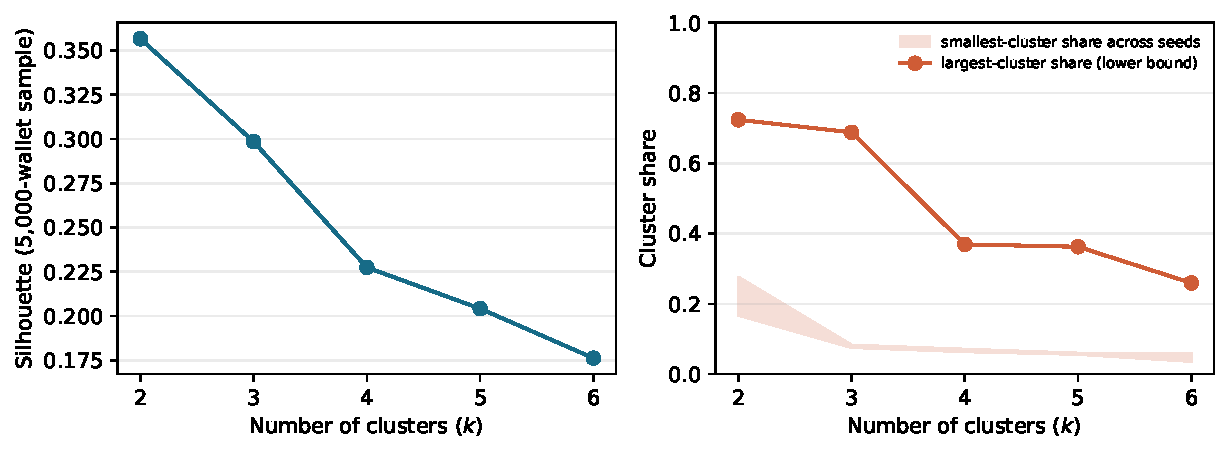
\includegraphics[width=\columnwidth]{figures/annual_model_resolution.pdf}
\caption{Annual resolution diagnostics. Silhouette is evaluated on the same 5,000-wallet sample; cluster-size ranges reflect the three seeds.}
\label{fig:resolution}\end{figure}
\begin{figure}[t]\centering
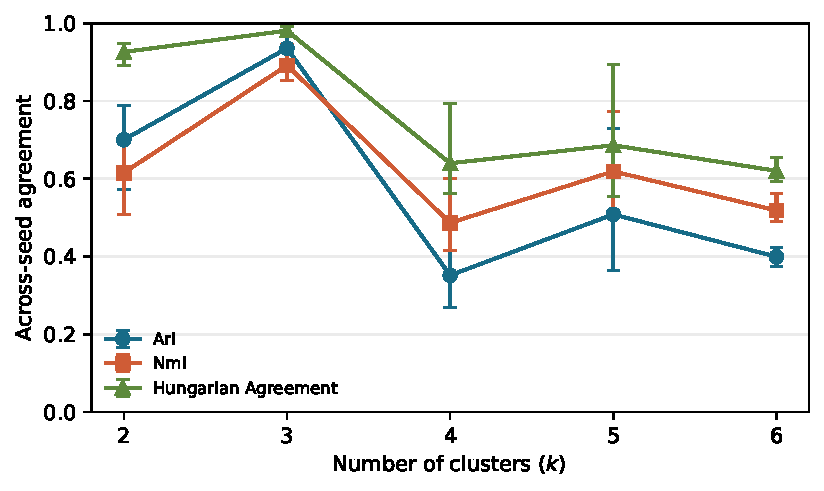
\includegraphics[width=\columnwidth]{figures/annual_seed_stability.pdf}
\caption{Full-population seed agreement. Points show means over the three seed pairs and bars their minimum and maximum.}
\label{fig:stability}\end{figure}

\subsection{Static K3 Behavioural Profiles}
The sustained-activity group contains 572,750 addresses. Its median history has 29 active days, 73 transfer records and a 268-day span. The distributed lower-activity group contains 1,746,310 addresses, with medians of nine active days, sixteen transfers and a 173-day span. The short-span concentrated group contains 189,937 addresses, with four active days, sixteen transfers and a seven-day span. The distinction between the latter two groups is consequently not a simple ordering by transfer total.

The short-span group's median activity density is 0.75 and its concentration ratio is 0.50. These values describe a compact period with activity on a large fraction of days within that span and a substantial share of transfers concentrated on a peak day. The sustained group's median density is approximately 0.139 and concentration 0.116, while the distributed lower-activity group's values are approximately 0.060 and 0.211. An address can therefore be denser within a short span without being more persistent across the year.

@@PROFILE_TABLE@@

The profile names do not identify an application or controller. Medians describe distributions with overlap, not every address in a group. Interquartile ranges remain in the replication tables. Figure~\ref{fig:profiles} uses a common display scale; Table~\ref{tab:profiles} preserves raw units.

\begin{figure}[t]\centering
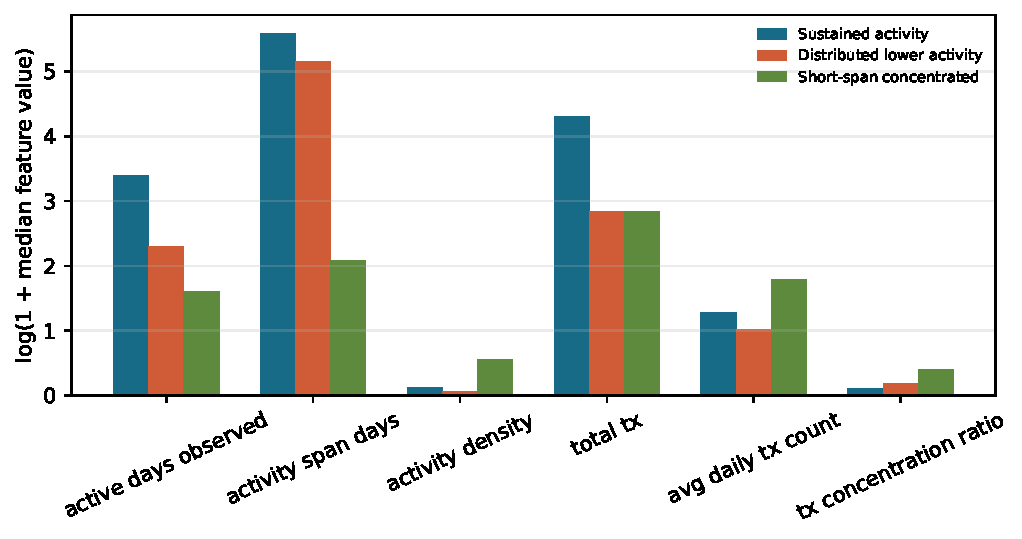
\includegraphics[width=\columnwidth]{figures/k3_count_activity_profiles.pdf}
\caption{Selected annual K3 median profiles. The display uses log(1+median) to put counts and ratios in one plot; the fit uses the documented feature-specific transformations.}
\label{fig:profiles}\end{figure}

\subsection{Feature Holdout Robustness}
Matched-estimator holdouts show that seed stability should not be confused with representation invariance. Removing activity-level features produces ARI 0.393 and matched agreement 0.780. Removing directionality produces ARI 0.711 and agreement 0.909. Removing persistence/concentration produces ARI 0.357 and agreement 0.595. NMI provides a complementary comparison in Table~\ref{tab:holdouts}. All comparisons use the same full-feature seed-492 reference and retain scaling for the surviving columns.

The persistence/concentration removal is consequential for an interpretation built around sustained and short-span activity, but activity removal also changes the partition substantially. The closer directionality holdout does not establish causal irrelevance. K3 summarizes the combined representation.

@@HOLDOUT_TABLE@@
\begin{figure}[t]\centering
\includegraphics[width=\columnwidth]{figures/matched_feature_holdouts.pdf}
\caption{Annual K3 sensitivity after removing each declared family, with the same estimator and fitting settings as the reference. Higher agreement means closer recovery of the full-feature partition.}
\label{fig:holdouts}\end{figure}

\subsection{Network Validation Across Annual Resolutions}
The twelve monthly files contain 38,733,517 transfer rows with two retained cohort endpoints. This is approximately 15.75\% of all processed transfer rows when months are pooled, with monthly coverage ranging from 13.7\% to 19.3\%. The exact counts describe the complete eligible subgraph before sampling. Each monthly permutation experiment then uses 200,000 eligible rows shared by every candidate solution, so resolution comparisons are not driven by different sampled interactions.

For annual K3 seed 492, sampled same-label fractions range from 0.503 to 0.601, with a mean of approximately 0.558. Null means range from 0.415 to 0.482, averaging approximately 0.468. The mean excess is 9.09 percentage points, with a monthly range of 2.99--13.32 points. All twelve tests have raw p-values of 0.0001, the resolution floor with 9,999 permutations, and Holm-adjusted values of 0.0084 within the 84-test family. These finite permutation values are not exact probabilities of zero.

@@NETWORK_TABLE@@

K4 seed 492 has larger mean network excess, 14.19 percentage points, and twelve supported months. K5 also has twelve supported months, with mean excess 8.35 points. K2 has three supported months but a negative average excess of approximately $-0.94$ points, while K6 has no supported upper-tail months and mean excess approximately $-3.83$ points. The direction and magnitude vary by resolution; adding groups does not monotonically improve this statistic. Nonsignificance for K6 does not establish that its partition is meaningless in every other respect.

K4 is not automatically preferred: its larger network excess accompanies lower annual seed stability, and activity--degree associations can affect this null. Network alignment remains a separate diagnostic rather than an independent utility score. K3 is selected for a readable, reproducible annual vocabulary.

\subsection{Network Sensitivity to K3 Initialization}
The additional K3 seeds also have supported upper-tail results in all twelve months after the same 84-test correction. Their mean excesses are 8.40 percentage points for seed 493 and 9.54 points for seed 494, compared with 9.09 for seed 492. Their monthly trajectories are similar but not identical. Figure~\ref{fig:networkcomparison} displays both the resolution comparison and the initialization comparison using shared monthly interactions, making the latter a test of label variation rather than a change in sampled edges.

\begin{figure*}[t]\centering
\includegraphics[width=0.95\textwidth]{figures/network_comparison_overview.pdf}
\caption{Annual network excess on shared monthly samples. Left: K2--K6 at seed 492. Right: the three K3 initializations. The null fixes transfer rows and shuffles endpoint-wallet labels; negative differences are descriptive under the declared upper-tail test.}
\label{fig:networkcomparison}\end{figure*}

\subsection{Held-Out Monthly Transitions}
The five held-out adjacent pairs contain 676,741--786,661 addresses active in both months. For monthly K3, observed persistence ranges from 0.639 to 0.702, compared with marginal-frequency chance agreement of 0.491--0.539. Kappa ranges from 0.292 to 0.353. These values describe moderate additional agreement beyond the chance baseline, not complete persistence. They are conditional on pairwise activity and should not be read as the fraction of the entire year-end cohort that remains in a state across every month.

The pooled K3 transition matrix also shows heterogeneity among monthly states. Its diagonal entries are approximately 0.775, 0.486 and 0.526 for monthly states 0, 1 and 2. The corresponding off-diagonal entries indicate substantial movement, including a probability of approximately 0.468 from state 1 to state 0. These numerical identifiers refer only to the frozen monthly model. They must not be matched by number to the sustained, distributed and short-span annual groups, because the feature spaces and centroids are different.

@@PERSISTENCE_TABLE@@
\begin{figure}[t]\centering
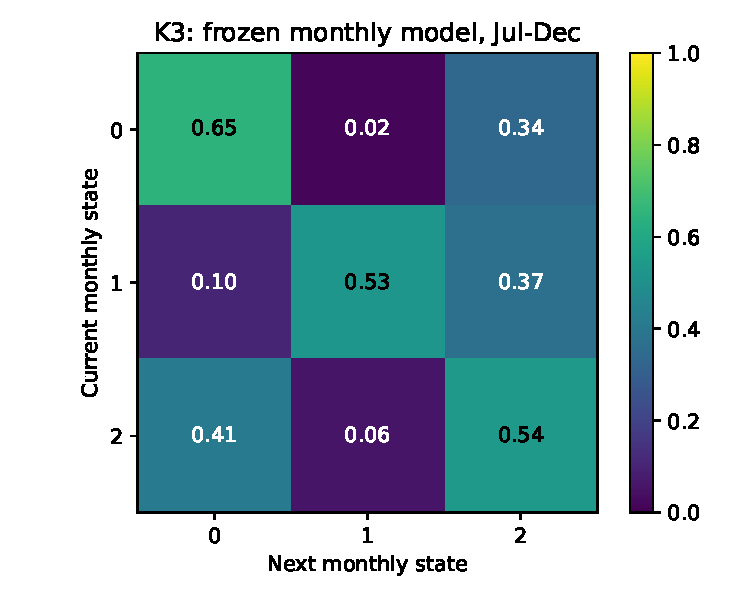
\includegraphics[width=0.92\columnwidth]{figures/k3_heldout_transition_matrix.pdf}
\caption{Pooled held-out transition probabilities for frozen monthly K3. States are assigned only to active wallet-months; monthly and annual IDs are distinct.}
\label{fig:monthlymatrix}\end{figure}

\subsection{Monthly Resolution Comparison}
Monthly K2 has the highest raw persistence, 0.797--0.831, but also the highest chance baseline, 0.653--0.693. Its kappa range, 0.415--0.448, is larger than that of K3. The monthly analysis therefore does not establish K3 as an optimal temporal resolution. K3 is the main illustration because it provides a compact state vocabulary alongside the annual study, while the full K2--K6 comparison is retained to expose the effects of granularity. Choosing a monthly resolution requires its own application-dependent objective.

Across K4--K6, raw persistence decreases with granularity, but every adjacent pair remains above marginal chance. Figure~\ref{fig:monthlyresolutions} shows that the excess-persistence curves are closer than raw fractions suggest. A finer partition can expose changes that a coarser one combines.

\begin{figure}[t]\centering
\includegraphics[width=\columnwidth]{figures/monthly_resolution_comparison.pdf}
\caption{Held-out persistence above marginal chance for independently trained monthly K2--K6 models on shared count-only inputs. The horizontal axis enumerates July--August through November--December.}
\label{fig:monthlyresolutions}\end{figure}

\subsection{Conditional Two-Step Return Behaviour}
Among first-step switchers, K3 observed return ranges from 0.409 to 0.471 across the four held-out triples. The conditional null means range from 0.383 to 0.448. The excess is approximately 1.88--2.58 percentage points. All four raw permutation p-values are 0.001 and all four adjusted values are 0.020 after correction across the twenty temporal tests. Table~\ref{tab:returns} gives the K3 triple-specific denominators and effects so that statistical support is not mistaken for a large unconditional return probability.

@@RETURN_TABLE@@

K4--K6 also have four supported return triples each. Their excess ranges are approximately 3.61--5.07, 4.16--5.81 and 4.98--6.15 percentage points, respectively. These larger effects are conditional on each model's own switcher set and state definitions. They do not form a direct same-population ranking of temporal predictive performance. In particular, finer partitions change both the opportunity to switch and the meaning of returning, even though the underlying wallet-month feature inputs are shared.

@@RETURN_SUMMARY_TABLE@@
\begin{figure}[t]\centering
\includegraphics[width=\columnwidth]{figures/conditional_return_comparison.pdf}
\caption{Conditional return excess for monthly K3--K6 over four held-out triples. K2 is omitted from the curves because its within-middle-state return null is structurally constant.}
\label{fig:returncomparison}\end{figure}

For K2, the observed return statistic equals every permuted statistic apart from numerical averaging precision, yielding p-values of one. This is expected from the binary switcher constraint, not evidence of absent temporal organization. Keeping the degeneracy explicit is important because a naive table of significant tests would otherwise make K2 appear to fail a test that has no power to distinguish the relevant behaviour. The finding illustrates why understanding a null's conditional structure matters as much as obtaining a small p-value.

\section{Discussion}
\subsection{What Makes the Annual K3 Interpretation Defensible}
The strongest case for K3 combines several qualified observations. Its annual labels are substantially more stable across the tested seeds than the finer alternatives. Its profiles distinguish duration and concentration in addition to count magnitude. Its network alignment persists across three initializations and twelve months under the shared-label null. These properties make it a practical descriptive summary for this representation. None establishes that the population contains three intrinsic or permanent classes, and the feature holdouts directly argue against such an interpretation.

K4 prevents an overly favourable interpretation of K3: stronger average network alignment coexists with weaker initialization stability. Different objectives could therefore favour different working resolutions. Our choice values reproducible feature profiles as well as interaction evidence.

\subsection{Annual Roles and Monthly States Answer Different Questions}
The annual analysis aggregates a full year of activity into sixteen features, whereas the monthly analysis learns six within-month count features from a restricted training period. The monthly results demonstrate persistence and history-dependent return within that separate representation. They do not show that an address moves between annual role labels or validate a one-to-one correspondence between the two taxonomies. Establishing such a correspondence would require an explicitly aligned analysis, not an assumption that equal numerical IDs have equal meaning.

\subsection{Representation and Population Boundaries}
Removing pooled token amounts is a substantive restriction, not a universal solution to measurement ambiguity. Counts describe emitted transfer activity in the supplied release; they do not measure comparable economic value across tokens. Incoming/outgoing day summaries do not determine ownership, intent or profitability. A future token-aware economic analysis would need a separate normalization strategy and validation of that strategy before attaching value-flow labels to the present groups. Reintroducing the older amount-based conclusions would undo the current representation control.

The historical cohort improves temporal specificity without proving continuous EOA status. It is a documented year-end subset of the supplied feature universe. The original selection of that universe is not independently reconstructed here; no prevalence estimate for all Ethereum users follows from these cluster shares. The membership changes demonstrate that present-day and historical code filters are not interchangeable.

\subsection{Network Dependence and the Meaning of External Evidence}
Network labels are tested on transfer endpoints rather than fitted through a graph objective, but the evidence is not independent of the activity representation. A frequent address contributes more opportunities to appear in the transfer sample, and activity-derived labels can correlate with degree or application exposure. The fixed-graph label shuffle breaks those associations. Consequently, a positive excess supports alignment under that randomization while leaving several mechanisms unresolved. Degree-stratified label nulls, token-specific analyses and additional sampling designs would provide complementary checks.

\subsection{Temporal Conditioning and Statistical Significance}
The monthly protocol improves separation between fitting and evaluation by freezing transformations and centroids before July--December assignment. Nevertheless, cohort selection uses a year-end observation, training samples are balanced by month, and evaluation excludes absent observations. These are explicit conditions, not properties of a prospective deployment. The return test also conditions on switching at the first step. A supported return effect describes this selected group and conditional null; it is not the probability that any randomly selected wallet will leave and recover an annual role.

Effect sizes must accompany p-values. K3 return excess is about two percentage points despite corrected significance, and dominant states partly explain high raw persistence. Statistical support concerns a declared comparison, not necessarily practical importance or an optimal resolution.

\subsection{Reproducibility and Remaining Research Directions}
The workflow records input membership, ordering, transformations, model settings and output hashes, and it rejects invalid daily sources and incomplete result families. Deterministic sorting before training sampling removes a previously hidden source of variation. The reproduced annual labels that differ from archived hashes remain identified rather than silently presented as exact recoveries. These controls do not eliminate all numerical or design dependence, but they allow a reader to determine which objects were reproduced exactly and which were rerun under the documented runtime.

Three initialization seeds measure only a narrow source of uncertainty; they do not establish resampling stability. Further work should test additional years, token-aware economic representations, degree-aware network nulls, representation alternatives and resampling schemes. No competing clustering algorithm or independently labelled social outcome is evaluated. The contribution to computational social systems is therefore measurement and validation of address-level participation patterns in a digital interaction system, rather than identification of people, social influence or a new clustering algorithm. Claims about social mechanisms or downstream utility require evidence beyond the present descriptive case study.

\section{Conclusion}
This study examines Ethereum wallet segmentation as a hypothesis requiring layered validation. A complete historical scan defines 2,508,997 year-end code-free addresses, and a controlled count/activity/direction representation supports a reproducible annual K3 working summary. Matched feature holdouts show substantial dependence on activity and persistence/concentration measurements. Shared-sample network comparisons provide corrected support for K3, K4 and K5 across all twelve months, with K4 displaying stronger mean alignment but weaker initialization stability. Separately trained monthly K2--K6 models show above-chance persistence, and K3--K6 exhibit conditional two-step return after the declared temporal correction. The binary K2 return null is explicitly uninformative.

The contribution is a transparent description of a bounded population, not an identity-recovery method or universal taxonomy. Annual roles, monthly states and network alignment provide distinct evidence. Retaining their agreement, disagreement and inferential boundaries makes the segmentation auditable.

\section*{Code and Data Availability}
The project repository is \url{https://github.com/sudentrs/ethereum-wallet-behaviour-segmentation}. The accompanying replication record contains cohort membership, compact annual and monthly tables, network summaries, figures, source validation records and provenance manifests. Raw transfer files and large derived matrices are external to Git. The underlying ERC-20 Trading 2022 data are available from Harvard Dataverse \cite{somin2025erc2022,somin2025dataset}. All empirical claims use the controlled year-end pipeline; older experiments serve only as provenance.
